\documentclass[14pt,russian]{scrartcl}
\let\counterwithout\relax
\let\counterwithin\relax
\usepackage{lmodern}
\usepackage{float}
\usepackage{xcolor}
\usepackage{extsizes}
\usepackage{subfig}
\usepackage[export]{adjustbox}
\usepackage{tocvsec2} % возможность менять учитываемую глубину разделов в оглавлении
\usepackage[subfigure]{tocloft}

\usepackage{fancyvrb}
\usepackage{ulem,bm,mathrsfs,ifsym} %зачеркивания, особо жирный стиль и RSFS начертание
\usepackage{sectsty} % переопределение стилей подразделов
%%%%%%%%%%%%%%%%%%%%%%%

%%% Поля и разметка страницы %%%
\usepackage{pdflscape}                              % Для включения альбомных страниц
\usepackage{geometry}                               % Для последующего задания полей
\geometry{a4paper,tmargin=2cm,bmargin=2cm,lmargin=3cm,rmargin=1cm} % тоже самое, но лучше

%%% Математические пакеты %%%
\usepackage{amsthm,amsfonts,amsmath,amssymb,amscd}  % Математические дополнения от AMS
\usepackage{mathtools}                              % Добавляет окружение multlined
\usepackage[perpage]{footmisc}

%%%% Установки для размера шрифта 14 pt %%%%
%% Формирование переменных и констант для сравнения (один раз для всех подключаемых файлов)%%
%% должно располагаться до вызова пакета fontspec или polyglossia, потому что они сбивают его работу
%\newlength{\curtextsize}
%\newlength{\bigtextsize}
%\setlength{\bigtextsize}{13pt}
\KOMAoptions{fontsize=14pt}

\makeatletter
\def\showfontsize{\f@size{} point}
\makeatother

%\makeatletter
%\show\f@size                                       % неплохо для отслеживания, но вызывает стопорение процесса, если документ компилируется без команды  -interaction=nonstopmode 
%\setlength{\curtextsize}{\f@size pt}
%\makeatother

%шрифт times
\usepackage{tempora}

   %%% Решение проблемы копирования текста в буфер кракозябрами
%    \input glyphtounicode.tex
%    \input glyphtounicode-cmr.tex %from pdfx package
%    \pdfgentounicode=1
    \usepackage{cmap}                               % Улучшенный поиск русских слов в полученном pdf-файле
    \usepackage[T2A]{fontenc}                       % Поддержка русских букв
    \usepackage[utf8]{inputenc}                     % Кодировка utf8
    \usepackage[english, main=russian]{babel}            % Языки: русский, английский
%   \IfFileExists{pscyr.sty}{\usepackage{pscyr}}{}  % Красивые русские шрифты
%\renewcommand{\rmdefault}{ftm}
%%% Оформление абзацев %%%
\usepackage{indentfirst}                            % Красная строка
%\usepackage{eskdpz}

%%% Таблицы %%%
\usepackage{longtable}                              % Длинные таблицы
\usepackage{multirow,makecell,array}                % Улучшенное форматирование таблиц
\usepackage{booktabs}                               % Возможность оформления таблиц в классическом книжном стиле (при правильном использовании не противоречит ГОСТ)

%%% Общее форматирование
\usepackage{soulutf8}                               % Поддержка переносоустойчивых подчёркиваний и зачёркиваний
\usepackage{icomma}                                 % Запятая в десятичных дробях



%%% Изображения %%%
\usepackage{graphicx}                               % Подключаем пакет работы с графикой
\usepackage{wrapfig}

%%% Списки %%%
\usepackage{enumitem}

%%% Подписи %%%
\usepackage{caption}                                % Для управления подписями (рисунков и таблиц) % Может управлять номерами рисунков и таблиц с caption %Иногда может управлять заголовками в списках рисунков и таблиц
%% Использование:
%\begin{table}[h!]\ContinuedFloat - чтобы не переключать счетчик
%\captionsetup{labelformat=continued}% должен стоять до самого caption
%\caption{}
% либо ручками \caption*{Продолжение таблицы~\ref{...}.} :)

%%% Интервалы %%%

%%% Счётчики %%%
\usepackage[figure,table,section]{totalcount}               % Счётчик рисунков и таблиц
\DeclareTotalCounter{lstlisting}
\usepackage{totcount}                               % Пакет создания счётчиков на основе последнего номера подсчитываемого элемента (может требовать дважды компилировать документ)
\usepackage{totpages}                               % Счётчик страниц, совместимый с hyperref (ссылается на номер последней страницы). Желательно ставить последним пакетом в преамбуле

%%% Продвинутое управление групповыми ссылками (пока только формулами) %%%
%% Кодировки и шрифты %%%

%   \newfontfamily{\cyrillicfont}{Times New Roman}
%   \newfontfamily{\cyrillicfonttt}{CMU Typewriter Text}
	%\setmainfont{Times New Roman}
	%\newfontfamily\cyrillicfont{Times New Roman}
	%\setsansfont{Times New Roman}                    %% задаёт шрифт без засечек
%	\setmonofont{Liberation Mono}               %% задаёт моноширинный шрифт
 %   \IfFileExists{pscyr.sty}{\renewcommand{\rmdefault}{ftm}}{}
%%% Интервалы %%%
%linespread-реализация ближе к реализации полуторного интервала в ворде.
%setspace реализация заточена под шрифты 10, 11, 12pt, под остальные кегли хуже, но всё же ближе к типографской классике. 
\linespread{1.3}                    % Полуторный интервал (ГОСТ Р 7.0.11-2011, 5.3.6)
%\renewcommand{\@biblabel}[1]{#1}

%%% Гиперссылки %%%
\usepackage{hyperref}

%%% Выравнивание и переносы %%%
\sloppy                             % Избавляемся от переполнений
\clubpenalty=10000                  % Запрещаем разрыв страницы после первой строки абзаца
\widowpenalty=10000                 % Запрещаем разрыв страницы после последней строки абзаца

\makeatletter % малые заглавные, small caps shape
\let\@@scshape=\scshape
\renewcommand{\scshape}{%
  \ifnum\strcmp{\f@series}{bx}=\z@
    \usefont{T1}{cmr}{bx}{sc}%
  \else
    \ifnum\strcmp{\f@shape}{it}=\z@
      \fontshape{scsl}\selectfont
    \else
      \@@scshape
    \fi
  \fi}
\makeatother

%%% Подписи %%%
%\captionsetup{%
%singlelinecheck=off,                % Многострочные подписи, например у таблиц
%skip=2pt,                           % Вертикальная отбивка между подписью и содержимым рисунка или таблицы определяется ключом
%justification=centering,            % Центрирование подписей, заданных командой \caption
%}
%%%        Подключение пакетов                 %%%
\usepackage{ifthen}                 % добавляет ifthenelse
%%% Инициализирование переменных, не трогать!  %%%
\newcounter{intvl}
\newcounter{otstup}
\newcounter{contnumeq}
\newcounter{contnumfig}
\newcounter{contnumtab}
\newcounter{pgnum}
\newcounter{bibliosel}
\newcounter{chapstyle}
\newcounter{headingdelim}
\newcounter{headingalign}
\newcounter{headingsize}
\newcounter{tabcap}
\newcounter{tablaba}
\newcounter{tabtita}
%%%%%%%%%%%%%%%%%%%%%%%%%%%%%%%%%%%%%%%%%%%%%%%%%%

%%% Область упрощённого управления оформлением %%%

%% Интервал между заголовками и между заголовком и текстом
% Заголовки отделяют от текста сверху и снизу тремя интервалами (ГОСТ Р 7.0.11-2011, 5.3.5)
\setcounter{intvl}{3}               % Коэффициент кратности к размеру шрифта

%% Отступы у заголовков в тексте
\setcounter{otstup}{0}              % 0 --- без отступа; 1 --- абзацный отступ

%% Нумерация формул, таблиц и рисунков
\setcounter{contnumeq}{1}           % Нумерация формул: 0 --- пораздельно (во введении подряд, без номера раздела); 1 --- сквозная нумерация по всей диссертации
\setcounter{contnumfig}{1}          % Нумерация рисунков: 0 --- пораздельно (во введении подряд, без номера раздела); 1 --- сквозная нумерация по всей диссертации
\setcounter{contnumtab}{1}          % Нумерация таблиц: 0 --- пораздельно (во введении подряд, без номера раздела); 1 --- сквозная нумерация по всей диссертации

%% Оглавление
\setcounter{pgnum}{0}               % 0 --- номера страниц никак не обозначены; 1 --- Стр. над номерами страниц (дважды компилировать после изменения)

%% Библиография
\setcounter{bibliosel}{1}           % 0 --- встроенная реализация с загрузкой файла через движок bibtex8; 1 --- реализация пакетом biblatex через движок biber

%% Текст и форматирование заголовков
\setcounter{chapstyle}{1}           % 0 --- разделы только под номером; 1 --- разделы с названием "Глава" перед номером
\setcounter{headingdelim}{1}        % 0 --- номер отделен пропуском в 1em или \quad; 1 --- номера разделов и приложений отделены точкой с пробелом, подразделы пропуском без точки; 2 --- номера разделов, подразделов и приложений отделены точкой с пробелом.

%% Выравнивание заголовков в тексте
\setcounter{headingalign}{0}        % 0 --- по центру; 1 --- по левому краю

%% Размеры заголовков в тексте
\setcounter{headingsize}{0}         % 0 --- по ГОСТ, все всегда 14 пт; 1 --- пропорционально изменяющийся размер в зависимости от базового шрифта

%% Подпись таблиц
\setcounter{tabcap}{0}              % 0 --- по ГОСТ, номер таблицы и название разделены тире, выровнены по левому краю, при необходимости на нескольких строках; 1 --- подпись таблицы не по ГОСТ, на двух и более строках, дальнейшие настройки: 
%Выравнивание первой строки, с подписью и номером
\setcounter{tablaba}{2}             % 0 --- по левому краю; 1 --- по центру; 2 --- по правому краю
%Выравнивание строк с самим названием таблицы
\setcounter{tabtita}{1}             % 0 --- по левому краю; 1 --- по центру; 2 --- по правому краю

%%% Рисунки %%%
\DeclareCaptionLabelSeparator*{emdash}{~--- }             % (ГОСТ 2.105, 4.3.1)
\captionsetup[figure]{labelsep=emdash,font=onehalfspacing,position=bottom}

%%% Таблицы %%%
\ifthenelse{\equal{\thetabcap}{0}}{%
    \newcommand{\tabcapalign}{\raggedright}  % по левому краю страницы или аналога parbox
}

\ifthenelse{\equal{\thetablaba}{0} \AND \equal{\thetabcap}{1}}{%
    \newcommand{\tabcapalign}{\raggedright}  % по левому краю страницы или аналога parbox
}

\ifthenelse{\equal{\thetablaba}{1} \AND \equal{\thetabcap}{1}}{%
    \newcommand{\tabcapalign}{\centering}    % по центру страницы или аналога parbox
}

\ifthenelse{\equal{\thetablaba}{2} \AND \equal{\thetabcap}{1}}{%
    \newcommand{\tabcapalign}{\raggedleft}   % по правому краю страницы или аналога parbox
}

\ifthenelse{\equal{\thetabtita}{0} \AND \equal{\thetabcap}{1}}{%
    \newcommand{\tabtitalign}{\raggedright}  % по левому краю страницы или аналога parbox
}

\ifthenelse{\equal{\thetabtita}{1} \AND \equal{\thetabcap}{1}}{%
    \newcommand{\tabtitalign}{\centering}    % по центру страницы или аналога parbox
}

\ifthenelse{\equal{\thetabtita}{2} \AND \equal{\thetabcap}{1}}{%
    \newcommand{\tabtitalign}{\raggedleft}   % по правому краю страницы или аналога parbox
}

\DeclareCaptionFormat{tablenocaption}{\tabcapalign #1\strut}        % Наименование таблицы отсутствует
\ifthenelse{\equal{\thetabcap}{0}}{%
    \DeclareCaptionFormat{tablecaption}{\tabcapalign #1#2#3}
    \captionsetup[table]{labelsep=emdash}                       % тире как разделитель идентификатора с номером от наименования
}{%
    \DeclareCaptionFormat{tablecaption}{\tabcapalign #1#2\par%  % Идентификатор таблицы на отдельной строке
        \tabtitalign{#3}}                                       % Наименование таблицы строкой ниже
    \captionsetup[table]{labelsep=space}                        % пробельный разделитель идентификатора с номером от наименования
}

\DeclareCaptionFormat{listings}{%
%\setlength{\fboxsep}{0pt}%
\parbox[top][0pt][l]{\textwidth}{\hspace{0pt}#1#2#3}}

\captionsetup[lstlisting]{justification=raggedright, singlelinecheck=off}

\captionsetup[table]{format=tablecaption,singlelinecheck=off,font=onehalfspacing,position=top,skip=-5pt, justification=raggedright}

\captionsetup[tabular]{format=tablecaption,singlelinecheck=off,font=onehalfspacing,position=top,skip=-5pt, justification=raggedright}

\DeclareCaptionLabelFormat{continued}{Продолжение таблицы~#2}
\setlength{\belowcaptionskip}{.2cm}
\setlength{\intextsep}{0ex}

%%% Подписи подрисунков %%%
\renewcommand{\thesubfigure}{\asbuk{subfigure}}           % Буквенные номера подрисунков
\captionsetup[subfigure]{font={normalsize},               % Шрифт подписи названий подрисунков (не отличается от основного)
    labelformat=brace,                                    % Формат обозначения подрисунка
    justification=centering,                              % Выключка подписей (форматирование), один из вариантов            
}
%\DeclareCaptionFont{font12pt}{\fontsize{12pt}{13pt}\selectfont} % объявляем шрифт 12pt для использования в подписях, тут же надо интерлиньяж объявлять, если не наследуется
%\captionsetup[subfigure]{font={font12pt}}                 % Шрифт подписи названий подрисунков (всегда 12pt)

%%% Настройки гиперссылок %%%

\definecolor{linkcolor}{rgb}{0.0,0,0}
\definecolor{citecolor}{rgb}{0,0.0,0}
\definecolor{urlcolor}{rgb}{0,0,0}

\hypersetup{
    linktocpage=true,           % ссылки с номера страницы в оглавлении, списке таблиц и списке рисунков
%    linktoc=all,                % both the section and page part are links
%    pdfpagelabels=false,        % set PDF page labels (true|false)
    plainpages=true,           % Forces page anchors to be named by the Arabic form  of the page number, rather than the formatted form
    colorlinks,                 % ссылки отображаются раскрашенным текстом, а не раскрашенным прямоугольником, вокруг текста
    linkcolor={linkcolor},      % цвет ссылок типа ref, eqref и подобных
    citecolor={citecolor},      % цвет ссылок-цитат
    urlcolor={urlcolor},        % цвет гиперссылок
    pdflang={ru},
}
\urlstyle{same}
%%% Шаблон %%%
%\DeclareRobustCommand{\todo}{\textcolor{red}}       % решаем проблему превращения названия цвета в результате \MakeUppercase, http://tex.stackexchange.com/a/187930/79756 , \DeclareRobustCommand protects \todo from expanding inside \MakeUppercase
\setlength{\parindent}{2.5em}                       % Абзацный отступ. Должен быть одинаковым по всему тексту и равен пяти знакам (ГОСТ Р 7.0.11-2011, 5.3.7).

%%% Списки %%%
% Используем дефис для ненумерованных списков (ГОСТ 2.105-95, 4.1.7)
%\renewcommand{\labelitemi}{\normalfont\bfseries~{---}} 
\renewcommand{\labelitemi}{\bfseries~{---}} 
\setlist{nosep,%                                    % Единый стиль для всех списков (пакет enumitem), без дополнительных интервалов.
    labelindent=\parindent,leftmargin=*%            % Каждый пункт, подпункт и перечисление записывают с абзацного отступа (ГОСТ 2.105-95, 4.1.8)
}
%%%%%%%%%%%%%%%%%%%%%%
%\usepackage{xltxtra} % load xunicode

\usepackage{ragged2e}
\usepackage[explicit]{titlesec}
\usepackage{placeins}
\usepackage{xparse}

\usepackage{listingsutf8}
\usepackage{url} %пакеты расширений
\usepackage{algorithm, algorithmicx}
\usepackage[noend]{algpseudocode}
\usepackage{blkarray}
\usepackage{chngcntr}
\usepackage{tabularx}
\newcommand*\template[1]{\text{<}#1\text{>}}

  
\titleformat{name=\section,numberless}[block]{\normalfont\Large\centering}{}{0em}{#1}
\titleformat{\section}[block]{\normalfont\Large\bfseries\raggedright}{}{0em}{\thesection\hspace{0.25em}#1}
\titleformat{\subsection}[block]{\normalfont\Large\bfseries\raggedright}{}{0em}{\thesubsection\hspace{0.25em}#1}
\titleformat{\subsubsection}[block]{\normalfont\large\bfseries\raggedright}{}{0em}{\thesubsubsection\hspace{0.25em}#1}

\let\Algorithm\algorithm
\renewcommand\algorithm[1][]{\Algorithm[#1]\setstretch{1.5}}

\usepackage{relsize}
\usepackage{pifont}
\usepackage{calc}
\usepackage{suffix}
\usepackage{csquotes}
\DeclareQuoteStyle{russian}
    {\guillemotleft}{\guillemotright}[0.025em]
    {\quotedblbase}{\textquotedblleft}
\ExecuteQuoteOptions{style=russian}
\newcommand{\enq}[1]{\enquote{#1}}  
\newcommand{\eng}[1]{\begin{english}#1\end{english}}
% Подчиненные счетчики в окружениях http://old.kpfu.ru/journals/izv_vuz/arch/sample1251.tex
\newcounter{cTheorem} 
\newcounter{cDefinition}
\newcounter{cConsequent}
\newcounter{cExample}
\newcounter{cLemma}
\newcounter{cConjecture}
\newtheorem{Theorem}{Теорема}[cTheorem]
\newtheorem{Definition}{Определение}[cDefinition]
\newtheorem{Consequent}{Следствие}[cConsequent]
\newtheorem{Example}{Пример}[cExample]
\newtheorem{Lemma}{Лемма}[cLemma]
\newtheorem{Conjecture}{Гипотеза}[cConjecture]

\renewcommand{\theTheorem}{\arabic{Theorem}}
\renewcommand{\theDefinition}{\arabic{Definition}}
\renewcommand{\theConsequent}{\arabic{Consequent}}
\renewcommand{\theExample}{\arabic{Example}}
\renewcommand{\theLemma}{\arabic{Lemma}}
\renewcommand{\theConjecture}{\arabic{Conjecture}}
%\makeatletter
\NewDocumentCommand{\Newline}{}{\text{\\}}
\newcommand{\sequence}[2]{\ensuremath \left(#1,\ \dots,\ #2\right)}

\definecolor{mygreen}{rgb}{0,0.6,0}
\definecolor{mygray}{rgb}{0.5,0.5,0.5}
\definecolor{mymauve}{rgb}{0.58,0,0.82}
\renewcommand{\listalgorithmname}{Список алгоритмов}
\floatname{algorithm}{Листинг}
\renewcommand{\lstlistingname}{Листинг}
\renewcommand{\thealgorithm}{\arabic{algorithm}}

\newcommand{\refAlgo}[1]{(листинг \ref{#1})}
\newcommand{\refImage}[1]{(рисунок \ref{#1})}

\renewcommand{\theenumi}{\arabic{enumi}.}% Меняем везде перечисления на цифра.цифра	
\renewcommand{\labelenumi}{\arabic{enumi}.}% Меняем везде перечисления на цифра.цифра
\renewcommand{\theenumii}{\arabic{enumii}}% Меняем везде перечисления на цифра.цифра
\renewcommand{\labelenumii}{(\arabic{enumii})}% Меняем везде перечисления на цифра.цифра
\renewcommand{\theenumiii}{\roman{enumiii}}% Меняем везде перечисления на цифра.цифра
\renewcommand{\labelenumiii}{(\roman{enumiii})}% Меняем везде перечисления на цифра.цифра
%\newfontfamily\AnkaCoder[Path=src/fonts/]{AnkaCoder-r.ttf}
\renewcommand{\labelitemi}{---}
\renewcommand{\labelitemii}{---}

%\usepackage{courier}

\graphicspath{ {./img/} }

\lstdefinelanguage{Refal}{
  alsodigit = {.,<,>},
  morekeywords = [1]{$ENTRY},
  morekeywords = [2]{Go, Put, Get, Open, Close, Arg, Add, Sub, Mul, Div, Symb, Explode, Implode},
  %keyword4
  morekeywords = [3]{<,>},
  %keyword5
  morekeywords = [4]{e.,t.,s.},
  sensitive = true,
  morecomment = [l]{*},
  morecomment = [s]{/*}{*/},
  commentstyle = \color{mygreen},
  morestring = [b]",
  morestring = [b]',
  stringstyle = \color{purple}
}

\makeatletter
\def\p@subsection{}
\def\p@subsubsection{\thesection\,\thesubsection\,}
\makeatother
\newcommand{\prog}[1]{{\ttfamily\small#1}}
\lstset{ %
  backgroundcolor=\color{white},   % choose the background color; you must add \usepackage{color} or \usepackage{xcolor}
  basicstyle=\ttfamily\footnotesize, 
  %basicstyle=\footnotesize\AnkaCoder,        % the size of the fonts that are used for the code
  breakatwhitespace=false,         % sets if automatic breaks shoulbd only happen at whitespace
  breaklines=true,                 % sets automatic line breaking
  captionpos=top,                    % sets the caption-position to bottom
  commentstyle=\color{mygreen},    % comment style
  deletekeywords={...},            % if you want to delete keywords from the given language
  escapeinside={\%*}{*)},          % if you want to add LaTeX within your code
  extendedchars=true,              % lets you use non-ASCII characters; for 8-bits encodings only, does not work with UTF-8
  inputencoding=utf8,
  frame=single,                    % adds a frame around the code
  keepspaces=true,                 % keeps spaces in text, useful for keeping indentation of code (possibly needs columns=flexible)
  keywordstyle=\bf,       % keyword style
  language=Refal,                    % the language of the code
  morekeywords={<,>,$ENTRY,Go,Arg, Open, Close, e., s., t., Get, Put}, 
  							       % if you want to add more keywords to the set
  numbers=left,                    % where to put the line-numbers; possible values are (none, left, right)
  numbersep=5pt,                   % how far the line-numbers are from the code
  xleftmargin=25pt,
  xrightmargin=25pt,
  numberstyle=\small\color{black}, % the style that is used for the line-numbers
  rulecolor=\color{black},         % if not set, the frame-color may be changed on line-breaks within not-black text (e.g. comments (green here))
  showspaces=false,                % show spaces everywhere adding particular underscores; it overrides 'showstringspaces'
  showstringspaces=false,          % underline spaces within strings only
  showtabs=false,                  % show tabs within strings adding particular underscores
  stepnumber=1,                    % the step between two line-numbers. If it's 1, each line will be numbered
  stringstyle=\color{mymauve},     % string literal style
  tabsize=4,                       % sets default tabsize to 8 spaces
  title=\lstname                   % show the filename of files included with \lstinputlisting; also try caption instead of title
}
\newcommand{\anonsection}[1]{\cleardoublepage
\phantomsection
\addcontentsline{toc}{section}{\protect\numberline{}#1}
\section*{#1}\vspace*{2.5ex} % По госту положены 3 пустые строки после заголовка ненумеруемого раздела
}
\newcommand{\sectionbreak}{\clearpage}
\renewcommand{\sectionfont}{\normalsize} % Сбиваем стиль оглавления в стандартный
\renewcommand{\cftsecleader}{\cftdotfill{\cftdotsep}} % Точки в оглавлении напротив разделов

\renewcommand{\cftsecfont}{\normalfont\large} % Переключение на times в содержании
\renewcommand{\cftsubsecfont}{\normalfont\large} % Переключение на times в содержании

\usepackage{caption} 
%\captionsetup[table]{justification=raggedleft} 
%\captionsetup[figure]{justification=centering,labelsep=endash}
\usepackage{amsmath}    % \bar    (матрицы и проч. ...)
\usepackage{amsfonts}   % \mathbb (символ для множества действительных чисел и проч. ...)
\usepackage{mathtools}  % \abs, \norm
    \DeclarePairedDelimiter\abs{\lvert}{\rvert} % операция модуля
    \DeclarePairedDelimiter\norm{\lVert}{\rVert} % операция нормы
\DeclareTextCommandDefault{\textvisiblespace}{%
  \mbox{\kern.06em\vrule \@height.3ex}%
  \vbox{\hrule \@width.3em}%
  \hbox{\vrule \@height.3ex}}    
\newsavebox{\spacebox}
\begin{lrbox}{\spacebox}
\verb*! !
\end{lrbox}
\newcommand{\aspace}{\usebox{\spacebox}}


\title{Lab 02 report}
\author{Kirill}

\date{\today}

\begin{document}
\thispagestyle{empty}

\noindent \begin{minipage}{0.15\textwidth}
	
\includegraphics[width=\linewidth]{b_logo}
\end{minipage}
\noindent\begin{minipage}{0.85\textwidth}\centering
	\textbf{Министерство науки и высшего образования Российской Федерации}\\
	\textbf{Федеральное государственное бюджетное образовательное учреждение высшего образования}\\
	\textbf{«Московский государственный технический университет имени Н.Э.~Баумана}\\
	\textbf{(национальный исследовательский университет)»}\\
	\textbf{(МГТУ им. Н.Э.~Баумана)}
\end{minipage}

\noindent\rule{16cm}{3pt}
\newline\newline
\noindent ФАКУЛЬТЕТ $\underline{\text{«Информатика и системы управления»}}$ \newline\newline
\noindent КАФЕДРА $\underline{\text{«Программное обеспечение ЭВМ и информационные технологии»}}$\newline


\begin{center}
	\noindent\begin{minipage}{1.3\textwidth}\centering
	\Large\textbf{   ~~~ Лабораторная работа №4}\newline
	\textbf{по дисциплине "Анализ Алгоритмов"}\newline\newline\newline
	\end{minipage}
\end{center}

\noindent\textbf{Тема} $\underline{\text{Параллельное программирование}}$\newline\newline
\noindent\textbf{Студент} $\underline{\text{Рядинский К. В.}}$\newline\newline
\noindent\textbf{Группа} $\underline{\text{ИУ7-53Б}}$\newline\newline
\noindent\textbf{Преподаватель} $\underline{\text{Волкова Л. Л.}}$\newline

\begin{center}
	\mbox{}
	\vfill
	Москва
\end{center}

\begin{center}
	\the\year ~г.
\end{center}
\clearpage

\renewcommand\contentsname{\hfill{\normalfont{СОДЕРЖАНИЕ}}\hfill}  %Оглавление
\tableofcontents
\newpage

\anonsection{Введение}

Параллельные вычисления часто используются для увеличения скорости выполнения
программ. Однако приемы, применяемые для однопоточных машин, для
параллельных могут не подходить.

В данной лабораторной работе будет рассмотрено и реализованно параллельное
программирование на примере задачи вычисления среднего арифметического строки матрицы.

Целью данной работы является изучения параллельных вычислений на материале
задачи вычисления среднего арифметического строки матрицы.

В рамках выполнения работы необходимо решить следующие задачи:

\begin{enumerate}
	\item Изучения основ параллельных вычислений.
	\item Выбор и обоснование языка программирования, для решения данной задачи.
	\item Применение изученных основ для реализации многопоточности на материале задачи вычисления среднего арифметического строки матрицы.
	\item Получения практических навыков.
	\item Сравнительный анализ параллельной и однопоточной реализации алгоритма вычисления среднего арифметического строки матрицы.
	\item Экспериментальное подтверждение различий во временной эффективности реализации однопоточной и многопоточной версии вычисления среднего арифметического строки матрицы.
	\item Описание и обоснование полученных результатов.
\end{enumerate}


\section{Аналитическая часть}

В данном разделе будут рассмотрены алгоритм вычисления среднего арифметического строки матрицы и его параллельная реализиация.

\subsection{Алгоритм вычисления среднего арифметического строки матрицы}

Данный алгоритм создал для вычисления среднего арифметичского строки матрицы следующим образом: для каждой вычисляется ее сумма и делится на длину \footnote{Длиной строки мы будем называть количество элементов принадлежащей этой строке} этой строки.

\begin{equation}
    \bar{A_i} = \frac{\displaystyle\sum_{j = 1}^{n} A_{i, j}}{n}, i = \overline{1, m}
\end{equation}

\subsection{Параллельная реализация вычисления среднего арифметического строки матрицы}

Посколько в рассмотренном выше алгоритме каждая строка обрабатывается независимо, появляется возможность распределить обработку строк среди потоков.

\subsection{Вывод}

В данном разделе были рассмотрены алгоритм вычисления среднего арифметического строки матрицы и его параллельная реализиация.

\section{Конструкторская часть}

В данном разделе будут представлены схемы алгоритмов (\ref{img:iter}-\ref{img:parallel}) и схемы вспомогательных функций (\ref{img:worker}-\ref{img:row_mean})). Описаны используемые типы данных, структура программного обеспечения (далее ПО) и классы эквивалентности.

\subsection{Схемы алгоритмов}

\begin{figure}[H]
    \centering
    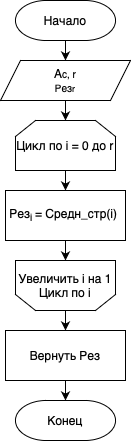
\includegraphics[scale=0.8]{iter.png}
    \caption{Схема последовательного алгоритма}
    \label{img:iter}
\end{figure}

\begin{figure}[H]
    \centering
    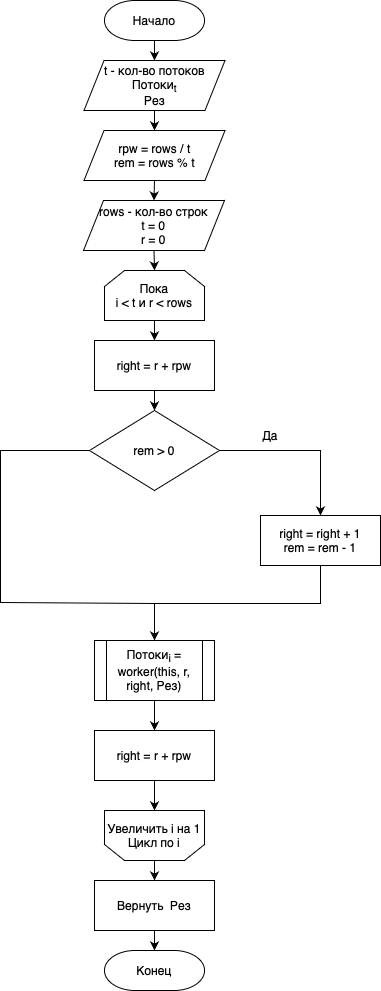
\includegraphics[scale=0.7]{parallel.png}
    \caption{Схема параллельного алгоритма}
    \label{img:parallel}
\end{figure}

\begin{figure}[H]
    \centering
    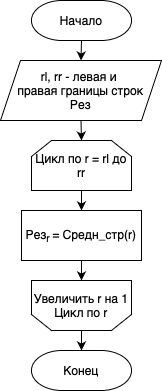
\includegraphics[scale=1]{worker.png}
    \caption{Схема вспомогательной функции worker}
    \label{img:worker}
\end{figure}

\begin{figure}[H]
    \centering
    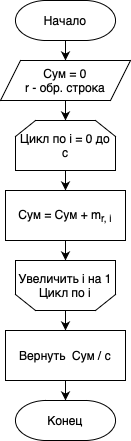
\includegraphics[scale=1]{row_mean.png}
    \caption{Схема вспомогательной функции вычисления среднего арифметического строки}
    \label{img:row_mean}
\end{figure}


\subsection{Описание используемых типов данных}

При реализации алгоритмов будут использованы следующие структуры данных:

\begin{enumerate}
	\item Матрица --- одномерный массив типа float.
	\item Количество строк матрицы --- целое число типа long long.
	\item Количество столбцов матрицы --- целое число типа long long.
	\item Результирующий вектор --- одномерный массив типа float.
	\item Массив потоков --- одномерный массив типа std::thread.
\end{enumerate}

\subsection{Структура ПО}

ПО будет состоять из следующих модулей:

\begin{enumerate}
	\item main.cpp --- модуль, содержащий точку входа программы.
	\item matrix.cpp --- модуль, содержащий код алгоритмов нахождения среднего арифметического матрицы.
\end{enumerate}

\subsection{Способы тестирования и классы эквивалентности}

При тестировании алгоритмов была выбрана методика тестирования черным ящиком. Были выделены следующие классы эквивалентности:

\begin{enumerate}
	\item Матрица, заполненная случайными положительными числами.
	\item Матрица, заполненная построчно равными элементами.
	\item Матрица, содержащая один элемент.
	\item Пустая матрица.
\end{enumerate}

\subsection{Вывод}

В данном разделе были рассмотрены схемы алгоритмов (\ref{img:iter}-\ref{img:parallel}) и схемы вспомогательных функций (\ref{img:worker}-\ref{img:row_mean})). Описаны используемые типы данных, структура ПО, способы тестирования и классы эквивалентности.

\section{Технологическая часть}

В данном разделе приведены средства реализации и листинги кода.

\subsection{Средства реализации}

К языку программирования выдвигаются следующие требования:

\begin{enumerate}
	\item Возможность порождать системные потоки.
	\item Возможность производить замер времени выполнения части программы.
	\item Существуют среды разработки для этого языка.
\end{enumerate}

По этим требованиям был выбран язык программирования C++.

\subsection{Листинги кода}

\begin{lstlisting}[caption=Последовательный алгоритм, label=list:iter, language={}]
real row_mean(const Matrix &m, size_t r) {
	real acc = 0;

	for (size_t c = 0; c < m.getcols(); c++) {
		acc += m(r, c);
	}

	return acc / m.getcols();
}

std::vector<real> Matrix::rows_mean() {
	std::vector<real> res(rows);


	for (size_t i = 0; i < rows; i++) {
		res[i] = row_mean(*this, i);
	}

	return res;
}
\end{lstlisting}

\begin{lstlisting}[caption=Параллельный алгоритм, label=list:iter, language={}]
static real row_mean(const real *ptr, size_t l) {
    real acc = 0;

    for (size_t i = 0; i < l; i++) {
        acc += ptr[i];
    }

    return acc / l;
}

static void rows_worker(const Matrix &m, size_t rl, size_t rr, std::vector<real> &res) {
    for (size_t r = rl; r < rr; r++) {
        res[r] = row_mean(m.getdata().data() + (r * m.getcols()), m.getcols());
    }
}

std::vector<real> Matrix::rows_mean_parallel(size_t t_num) {
    std::vector<std::thread> threads(t_num);
    std::vector<real> res(rows);

    size_t rpw       = rows / t_num; // rows per thread
    size_t remainder = rows % t_num;

    size_t t = 0;
    size_t r = 0;

    while (t < t_num && r < rows) {
        size_t right = r + rpw;

        if (remainder > 0) {
            right++;
            remainder--;
        }

        threads[t] = std::thread(rows_worker, std::cref(*this), r, right, std::ref(res));
        
        r = right;
        t++;
    }

    for (auto && i : threads) {
        i.join();
    }

    return res;
}
\end{lstlisting}

\subsection{Тестирование}

Тестирование проводилось методом черный ящик. \\

\begin{table}[ht]
	\caption{\centering Тестирование алгоритмов}
	\centering
	\begin{tabular}{|c|c|c|}
	\hline
	Ввод                                                          & Фактический результат & Ожидаемый результат \\ \hline
	1 2 3                                                         & 2                     & 2                   \\ \hline
	()                                                            & ()                    & ()                  \\ \hline
	0                                                             & 0                     & 0                   \\ \hline
	\begin{tabular}[c]{@{}c@{}}1 1 1\\ 2 2 2\\ 1 2 1\end{tabular} & 1, 2, 1.333333        & 1, 2, 1.333333      \\ \hline
	\end{tabular}
	\label{tab:tests}
	\end{table}

\subsection{Вывод}

В данном разделе были представлены средства реализации, листинги кода и проведено тестирование кода.

\section{Экспериментальная часть}

В данном разделе будет произведено сравнение временных характеристик вышеизложенных алгоритмов.

\subsection{Пример работы программы}

\begin{figure}[H]
    \centering
    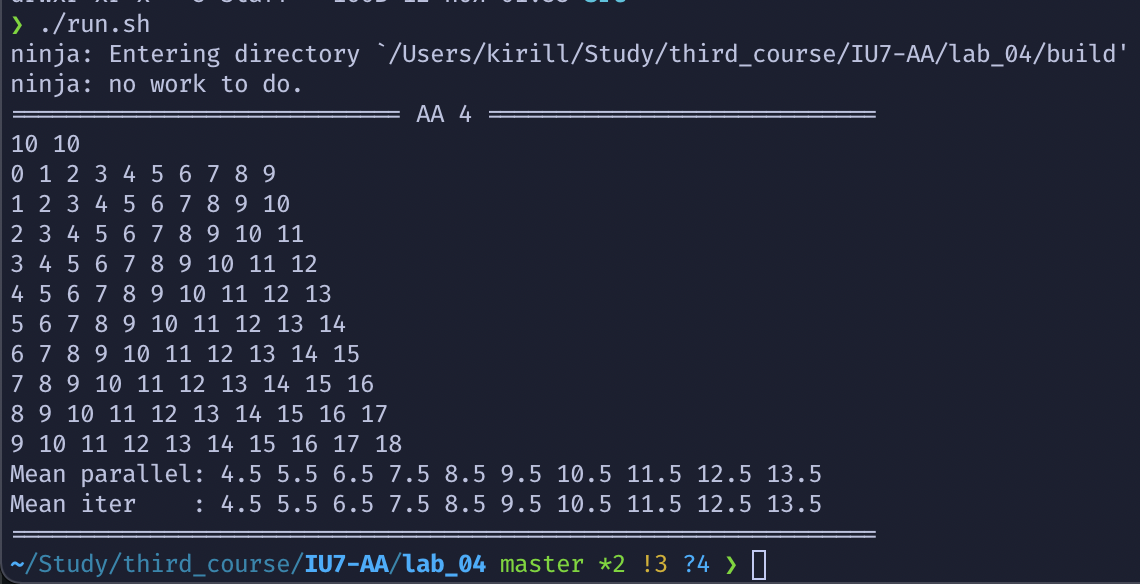
\includegraphics[scale=0.75]{example.png}
    \caption{Пример работы программы}
    \label{img:example}
\end{figure}

\subsection{Технические характеристики}

Технические характеристики электронно-вычислительнй машины, на которой выполнялось тестирование:

\begin{itemize}
    \item операционная система: macOS BigSur версия 11.4;
    \item оперативная память: 8 гигабайт LPDDR4;
    \item процессор: Apple M1.
\end{itemize}


Тестирование проводилось на ноутбуке, включенном в сеть электропитания. Во время тестирования ноутбук был нагружен только встроенными приложениями окружения рабочего стола, окружением рабочего стола, а также непосредственно системой тестирования.

\subsection{Временные характеристики}

Замер времени выполнения функций был произведен с помощью библиотеки Google Benchmark. Эта библиотека замеряет процессорное или реальное время (по выбору пользователя) выполнения функций, усредняет это значение и выдает результат в желаемом формате (csv, json, вывод в терминал).

\begin{figure}[H]
    \centering
    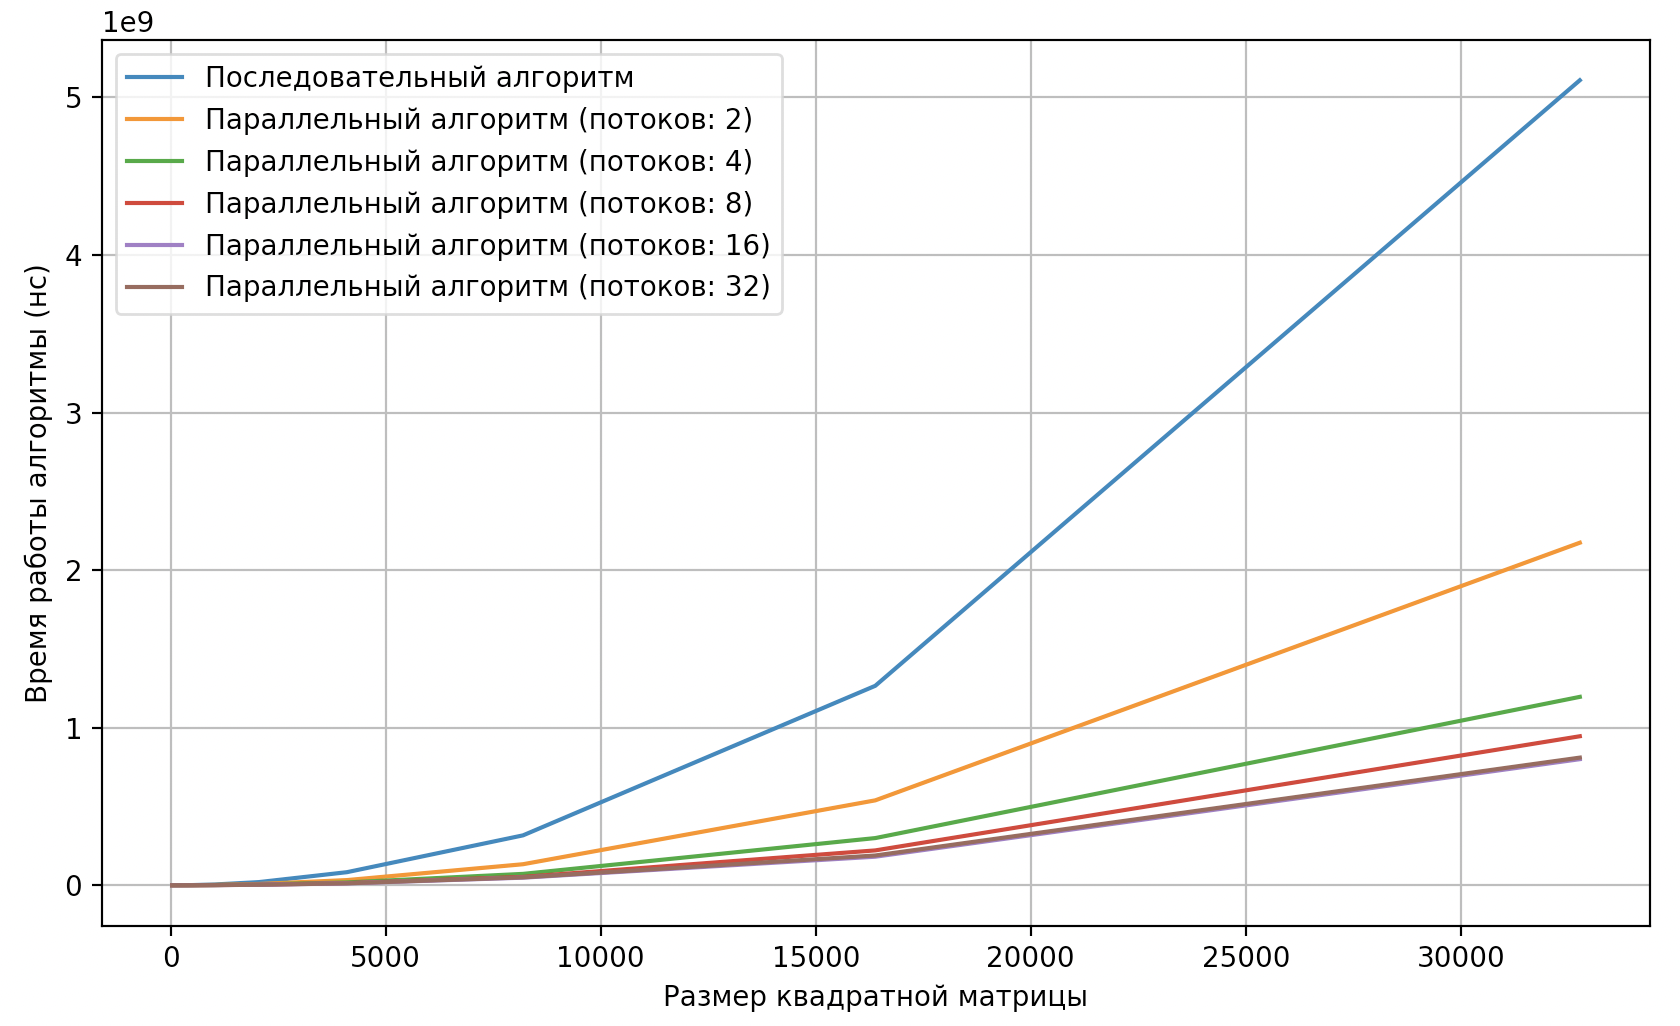
\includegraphics[scale=0.6]{plot.png}
    \caption{Зависимость времени выполнения алгоритма от размера квадратной матрицы}
    \label{img:benchmark}
\end{figure}

Как видно из графика \ref{img:benchmark}, параллельная реализация алгоритма быстрее последовательного как минимум в 2.5 раза для двух потоков. Также из графика видно, что для машины, на которой производилось тестирование, не имеет смысла порождать более 8 потоков, так как производительность почти не растет, но на создание потоков уходят ресурсы (память).

\subsection{Вывод}

В данном разделе было произведено сравнение реализаций алгоритмов и зависимость времени работы от количества потоков и сделаны соответствующие заключения.

\anonsection{Заключение}

В данной лабораторной работе были рассмотрены основополагающие материалы, которые в дальнейшем потребовались для параллельной и последовательной реализаций алгоритма вычисления среднего арифметического строки матрицы. 

В рамках данной лабораторной работы была достигнута цель и выполнены следующие задачи:

\begin{enumerate}
	\item Изучены основы параллельных вычислений.
	\item Выбран и обоснован язык программирования, для решения данной задачи.
	\item Примененены изученные основы для реализации многопоточности на материале задачи вычисления среднего арифметического строки матрицы.
	\item Получены практические навыки.
	\item Был проведен сравнительный анализ параллельной и однопоточной реализации алгоритма вычисления среднего арифметического строки матрицы.
	\item Было экспериментально подтверждено различия во временной эффективности реализации однопоточной и многопоточной версии вычисления среднего арифметического строки матрицы.
	\item Были описаны и обоснованы полученные результаты.
\end{enumerate}

\anonsection{Литература}

\begin{enumerate}
	\item Visual Studio Code [Электронный ресурс], режим доступа: https://code.visualstudio.com/ (дата обращения: \today)
	\item LPDDR4 [Электронный ресурс] \url{https://ru.wikipedia.org/wiki/LPDDR#LPDDR4} (дата обращения: \today)
	\item Ульянов М. В. Ресурсно-эффективные компьютерные алгоритмы. Разработка и Анализ. - Наука Физматлит, 2007. - 376.
\end{enumerate}

\end{document}
